\section{Analog-to-digital Converter}

As the name implies, an \emph{analog-to-digital converter}
(ADC) converts analog sound to a digital signal, like a
microphone.
\marginnote{An analog signal is continuous time and continuous
    amplitude, while a digital signal is discrete time and discrete
    amplitude}
The \emph{resolution} $N$ of an ADC is the number of binary bits
in the ADC output.

\begin{equation}
    \text{ADC Output} = round\left( (2^N - 1)\frac{V_{\text{input}}}{V_{\text{ref}}} \right)
\end{equation}

$V_{\text{ref}}$ is the maximum input voltage that can be converted by the ADC.

The least significant bit (LSB) holds the lowest value of the encoded
analog signal.
The maximum error due to quantization is
\begin{equation}
    \pm \frac{1}{2}LSB = \pm \frac{1}{2} \frac{V_\text{ref}}{2^N-1}
\end{equation}

An ADC does not have infinitely fast conversion. The \emph{sampling rate}
is the number of output samples available per unit time.

The sampling frequency needed to prevent aliasing, which causes distortion,
is given by the Nyquist-Shannon Sampling Theorem,
\begin{equation}
    f_{\text{sampling}} \geq 2f_{\text{signal}}
\end{equation}

This class focuses on \emph{successive-approximation} (SAR) ADCs,
as in Figure \ref{fig:saradc}.

\begin{figure}
    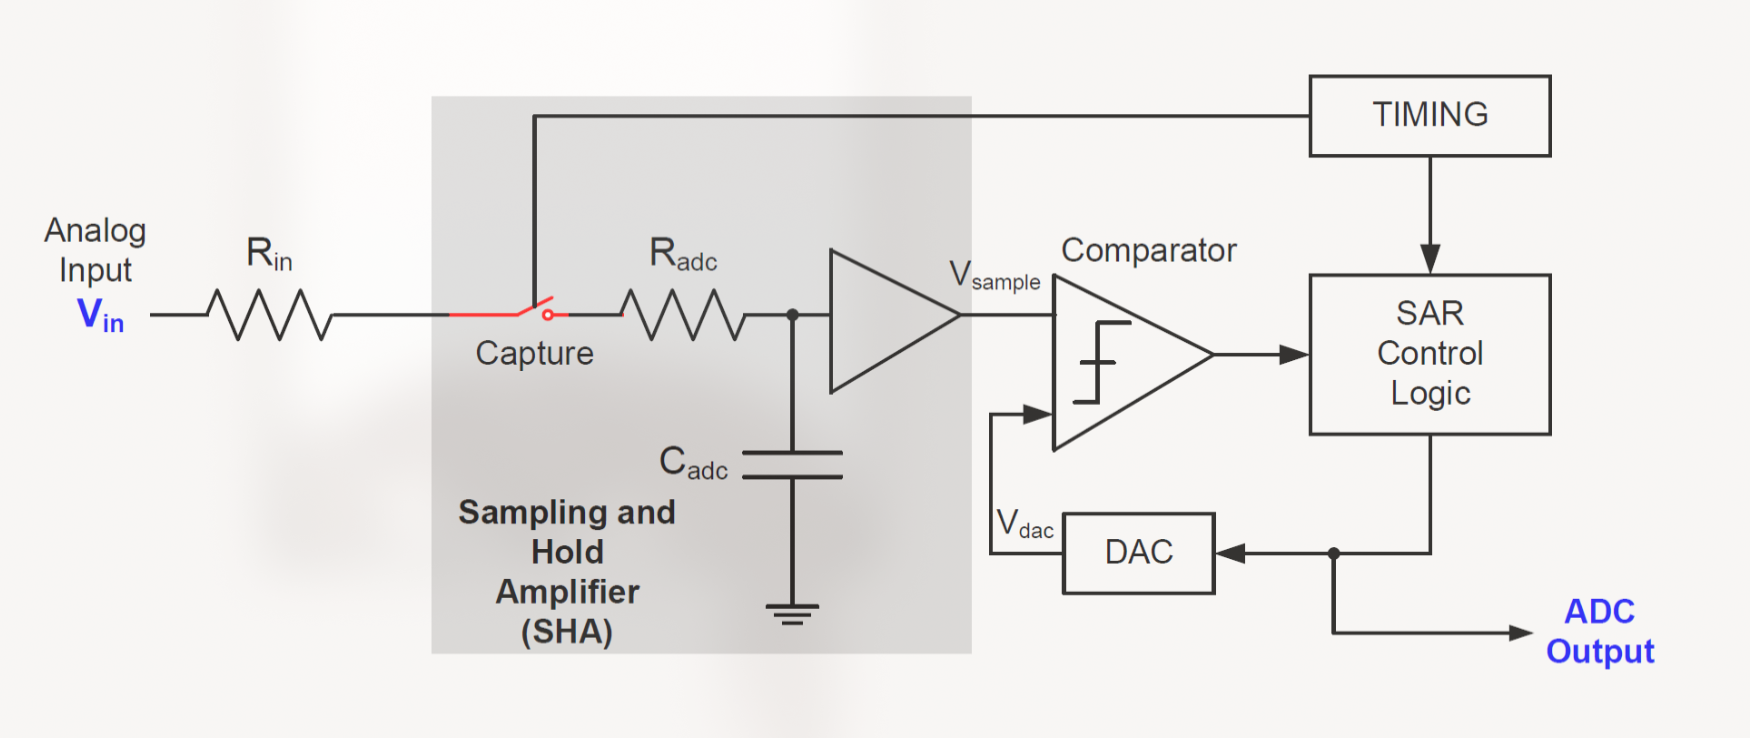
\includegraphics{images/saradc.png}
    \caption{SAR ADC}
    \label{fig:saradc}
\end{figure}